\documentclass{svmult}

\usepackage{mathptmx}
\usepackage{helvet}
\usepackage{courier}
\usepackage{makeidx}
\usepackage{multicol}

\usepackage{amsmath}
\usepackage{amssymb}
\usepackage{graphicx}
\usepackage[utf8]{inputenc}
%\usepackage{url}

\relax
\makeindex


\begin{document}

\title*{Modeling a Mobile Robot using a Grammatical Model}

\author{Gabriel L\'opez-Garc\'ia, 
		Javier Gallego-S\'anchez,  
		J. Luis Dalmau-Espert, \\
		Rafael Molina-Carmona 
		and Patricia Compa\~n-Rosique}

\authorrunning{G. L\'opez, 
			   J. Gallego, 
			   J.L. Dalmau, 
			   R. Molina
			   and P. Compa\~n}

\institute{Gabriel L\'opez-Garc\'ia, 
		Javier Gallego-S\'anchez,  
		J. Luis Dalmau-Espert,  
		Rafael Molina-Carmona 
		and Patricia Compa\~n-Rosique 
		\at 
		Grupo de Inform\'atica Industrial e Inteligencia Artificial, 
		Universidad de Alicante, Ap.99, E-03080, 
		Alicante, Spain
		\email{\{glopez, ajgallego, jldalmau, rmolina, patricia\}@dccia.ua.es}}

\maketitle


\abstract{
%Sensory multimodality is one of the capabilities of the human brain to fuse information from multiple sensors thus increasing the capacity of perception. Currently, robots simulate this capability from the information obtained by their multiple sensors as a way to improve the perception and the navigation ability.
%\newline\indent
Virtual Worlds Generator is a grammatical model that is proposed to define virtual worlds. It integrates the diversity of sensors and interaction devices, multimodality and a virtual simulation system. Its grammar allows the definition and abstraction in symbols strings  of the scenes of the virtual world, independently of the hardware that is used to represent the world or to interact with it.
\newline\indent
A case study is presented to explain how to use the proposed model to formalize a robot navigation system with multimodal perception and a hybrid control scheme of the robot.
}


%___________________________________________________________________________
\section{Introduction
\label{sec:introduction}}
%___________________________________________________________________________

Autonomous robots are physical agents that perform tasks by navigating in an environment and by manipulating objects in it. To perform these tasks, they are equipped with effectors to act on the environment (wheels, joints...) and with sensors that can perceive it (cameras, sonars...) \cite{Russell2010}. 

The growing disparity of available sensors adds complexity to systems, but it also allows the control of robots to be more accurate. For example, humans and other animals integrate multiple senses \cite{Sharma1998}. There are other reasons of mathematical nature: combining multiple observations from the same source provides statistical advantages because some redundant observations are obtained for the same estimation.

%Combining data from different sensors is an open field of research. This subject is dealt from different points of view. Signhal and Brown \cite{Singhal1997} consider that two main processes may be perform from several multimodal inputs: multisensor fusion (there is actual combination of different sources of information into one representation format) and multisensor integration (synergistic use of the information provided by multiple sensory devices to assist in the accomplishment of a task by a system). Other authors describe the evidence that humans combine information following two general strategies: The first one is to maximize information delivered from the different sensory modalities (combination). The second is to reduce the variance in the sensory estimate to increase its reliability (integration) \cite{Ernst2004}. 

In this paper we deal with the integration of multimodal inputs in the sense stated by Signhal and Brown \cite{Singhal1997}, that is, the use of data of different nature for decision-making in high-level tasks performed by a robot. However, the proposed system can also deal with the concept of fusion. 

%Different architectures have been described for defining the behaviour of a robot and the combination of sensory information. A robotic control architecture should have the following properties: programmability, autonomy and adaptability, reactivity, consistent behaviour, robustness and extensibility \cite{Ingrand2001}. To achieve those requirements, most robot architectures try to combine reactive control (guided by sensors) and deliberative control (global solutions can be obtained from the data collected by the sensors but also from information from an a priori model). They are, therefore, hybrid architectures \cite{Posadas2008}.

The Virtual Worlds Generator (VWG), our proposal, is a grammatical model, which integrates the diversity of interaction and sensing devices and the modules that make up a Graphics System (Graphics, Physics and AI engines). The scene definition is separated from the hardware-dependent characteristics of the system devices. It uses a grammar definition which integrates activities, visualization and interaction with users. The hypothesis is that it can be used as a formal framework to model a robot navigation system, including several multimodal inputs, sensor fusion and integration, and behaviour strategies.

%In section 2, the formal model for the VWG is presented. In section 3, the formal model is applied to construct a robotic system. Finally, some conclusions are presented in the last section.


%___________________________________________________________________________
\section{Model for Virtual Worlds Generation
\label{sec:model}}
%___________________________________________________________________________

In the VWG model, a virtual world is described as an ordered sequence of primitives, transformations and actors.
A primitive is the description of an object in a given representation system (typically, they are graphical primitives but they could also be sounds or any other primitive in a representation space).
Transformations modify the behaviour of primitives, and actors are the components which define the
activities of the system in the virtual world. The actors may be finally displayed through primitives and transformations. To model the different actor's activities, the concept of an event is used. Events cause the activation of a certain activity that can be processed by one or more actors.

Each element in the scene is represented by a symbol from the \textit{set of symbols of
the scene}. The symbols make up strings that describe the scenes, in accordance with a 
language syntax, which is presented as a grammar \cite{Davis1994}. 

%___________________________________________________________________________
%\subsection{Syntax
%\label{sec:semantic}}

A grammar $M$ is a tuple $M= \ <\Sigma, N, R, s>$, where $\Sigma$ is the finite set of
terminal symbols, $N$ is the finite set of non-terminal symbols, $R$ is the finite set of syntactic rules (a syntactic rule is an application $r$: $N \rightarrow W^*$, where $W = \Sigma \cup N$)
and $s \in N$ is the initial symbol of the grammar. In out case, $M$ is defined as:

\begin{enumerate}
    \item $\Sigma = P \cup T \cup O \cup A_{ATTR}^D$, where:

    \begin{itemize}
        \item $P$: set of symbols for primitives.

        \item $T$: set of symbols for transformations.

        \item $O = \{ \cdotp ( ) \}$: symbols for indicating the scope () and the concatenation $\cdotp$.

        \item $A_{ATTR}^D$: set of symbols for actors, where $D$ is the set of all the types of
        events generated by the system and $ATTR$ is the set of all the attributes of actors which define
        all the possible states. For example, the actor $a_{attr}^H$ will carry out its activity when it receives an
        event $e^h$, where $h \in H$, $H \subseteq D$ and $attr \in ATTR$ is its current state.
    \end{itemize}

    \item $N$ = \{WORLD, OBJECTS, OBJECT, ACTOR, TRANSFORM., FIGURE\}.

    \item Grammar rules $R$ are defined as:

		\begin{itemize}
			\item Rule 1. \textbf{WORLD} $\rightarrow$ OBJECTS
			\item Rule 2. \textbf{OBJECTS} $\rightarrow$ OBJECT $|$ OBJECT · OBJECTS
    		\item Rule 3. \textbf{OBJECT} $\rightarrow$ FIGURE $|$ TRANSFORM. $|$ ACTOR
			\item Rule 4. \textbf{ACTOR} $\rightarrow$ $a_{attr}^H$, $a_{attr}^H \in \textbf{A}_{ATTR}^D, H \subseteq D$
			\item Rule 5. \textbf{TRANSFORMATION} $\rightarrow t$(OBJECTS), $t \in T$
			\item Rule 6. \textbf{FIGURE} $\rightarrow$ $p^+$, $p \in P$ 
	    \end{itemize}

    \item $s =$ WORLD is the initial symbol of the grammar.

\end{enumerate}

$M$ is a context-free grammar. $L(M)$ is the language generated by the grammar $M$:
$L(M) = \lbrace w \in \Sigma^* \ | \ \text{WORLD} \stackrel{*}{\rightarrow} w \rbrace$


%___________________________________________________________________________
%\subsection{Semantics
%\label{sec:semantic}}

Apart from the language syntax, it is necessary to define the semantics of $L(M)$. It will be defined with a denotational method, that is, through mathematical functions. 

%___________________________________________________________________________
%\subsubsection{Semantic Function of Primitives (Rule 6)
%\label{sec:rule6}}

\textbf{Rule 6} defines a figure as a sequence of primitives. Primitive's semantics is defined as a function $\alpha: P \rightarrow G$. Each symbol in the set $P$ carries out a primitive on a given geometric
system $G$. So, depending on the definition of the function $\alpha$ and on the geometry of $G$, the result of
the system may be different. $G$ represents the actions to be run on a specific visual or
non-visual geometric system (e.g. the actions on OpenGL or on the system of a robot).
%TODO: ...........
The function $\alpha$ provides the abstraction needed to homogenize the
different implementations of a rendering system. Therefore, only a descriptive string is needed to
run the same scene on different systems.


%___________________________________________________________________________
%\subsubsection{Semantic Function of Transformations (Rule 5)
%\label{sec:rule5}}

In \textbf{Rule 5}, two functions are used to describe the semantics of a transformation, whose scope is limited by the symbols ``()'': $\beta: T \rightarrow G$ (carried out when the symbol ``('' is processed) and $\delta: T \rightarrow G$ (run when the symbol ``)'' is found). These two functions have the same features that the function $\alpha$, but they are applied to the set of transformations $T$, using the same geometric system
$G$.


%___________________________________________________________________________
%\subsubsection{Semantic Function of Actors (Rule 4)
%\label{sec:rule4}}

\textbf{Rule 4} refers to actors, which are the dynamic part of the system. The semantics
of the actor is a function which defines its evolution in time. For this reason, the semantic
function is called \textit{evolution function} $\lambda$ and it is defined as:
$\lambda: A_{ATTR}^D \times E^D \rightarrow L(M)$, 
where $E^D$ is the set of events for the set of all event types $D$. The function $\lambda$ has a different expression depending on its evolution. However, a
general expression can be defined. Let $H = \{ h_0, \ldots,h_n \} \subseteq D$ be the subset of
event types which the actor $a_{ATTR}^H$ is prepared to respond to. 
The general expression for $\lambda$ can be seen at (e1), 
where $u_0, \ldots, u_n$ are strings of $L(M)$. This equation means that an actor $a_{ATTR}^{H}$ can
evolve, that is, it is transformed into another string $u_i$ when it responds to an event $e^h$
which the actor is prepared to respond to. However, the actor remains unchanged when it is not
prepared to respond.

As well as dynamic elements, actors can also have a representation in the geometric space $G$. To be displayed, an actor must be converted to a string of primitives and transformations. 
This visualization function is defined as:
$\theta: A_{ATTR}^D \times E^V \rightarrow L(M')$, 
where $V \subseteq D$, $E^V \subseteq E^D$ are events created in the visualization process, and
$L(M')$ is a subset of the language $L(M)$, made up of the strings with no actors. Let $H \cap V =
\{ v_0, \ldots,v_n \} \subseteq D$ be the subset of visual event types which the actor $a_{ATTR}^H$ is
prepared to respond to. 
The expression of $\theta$ can be seen at (e2).


%\vspace{-0.4cm}

\begin{tabular} {p{0.4\linewidth}p{0.1\linewidth}|p{0.4\linewidth}p{0.1\linewidth}}

%\begin{equation}
    $
    \lambda (a_{ATTR}^{H}, e^{h})=
    $
    & 
	&
	\ \ $   
    \theta (a_{ATTR}^H, e^v) =
    $
    &

    \\
    
    $
    \left\{
    \begin{array}{ll}
        u_0 \in L(M) & \mathit{if}  \ \ h = h_0 \\
        \hdots \\
        u_n \in L(M) & \mathit{if}  \ \ h = h_n \\
        a_{ATTR}^{H}  & \mathit{if}  \ \ h \notin H
    \end{array}\right\}
    $
	&
	(e1)
	&
	\ \ 
	$
    \left\{
    \begin{array}{ll}
        z_0 \in L(M') & \mathit{if}  \ \ v = v_0 \\
        \hdots \\
        z_n \in L(M') & \mathit{if}  \ \ v = v_n \\
        \epsilon  & \mathit{if}  \ \ v \notin H \cap V
    \end{array}\right\}
    $
    &
    (e2)
%\end{equation}

\end{tabular}

%


%___________________________________________________________________________
%\subsubsection{Semantic Functions of OBJECT, OBJECTS and WORLD (R. 1, 2, 3)
%\label{sec:rules123}}

The semantic function of these \textbf{Rules 1, 2, and 3} breaks down the strings and converts them into substrings, executing the so called $algorithm \ of \ the \ system$, which performs the complete evolution of the system and displays it in the current geometric system. It performs several actions, which are described in the following paragraphs.

To display the scene on the geometric system $G$, the function $\varphi$ is defined, for the set of symbols that can directly be displayed:  primitives and transformations. Given a
string $w \in L(M)$ and using only symbols of $P$ and $T$, $\varphi$ is defined as:

\vspace{-0.4cm}
\[
    \varphi (w) = \left\{
    \begin{array}{ll}
        \alpha(w) & \mathit{if} \ w \in P  \\

        \beta(t); \varphi(v); \delta(t) & \mathit{if} \ w = t(v) \wedge v \in L(M) \wedge \ t \in T \\

        \varphi(u); \varphi(v)  & \mathit{if} \ w = u \cdotp v \wedge u, v \in L(M)
    \end{array}\right\}
\]

In the case of strings including both displayable elements, and actors, two functions must be defined. The first one is the so called \textit{function of the system evolution} $\eta$, which requires
a sequence of sorted events $S = e^1 \cdot e^2 \dots e^n$, where every $e^i \in E^D$ and a string of $L(M)$ including actors, and implements a set of recursive calls to the function $\lambda$ to perform the evolution of all the actors in the system at a given frame:

\vspace{-0.4cm}
\[
    \eta (w, S) = \left\{
    \begin{array}{ll}
        w   & \mathit{if}  \ \ w \in P \\

        t(\eta (v, S))    & \mathit{if}  \ \  w = t(v)  \\

        \prod_{e^{i} \in S} \lambda (a_{attr}^H, e^i)    & \mathit{if}  \ \ w = a_{attr}^H \\

        \eta (u, S) \cdot \eta (v, S)   & \mathit{if}  \ \  w = u \cdot v
    \end{array}\right\}
\]

The operator $\prod_{e^{i} \in S} \lambda (a_{attr}^H, e^i)$ concatenates the strings of the function $\lambda$. 

For the actors to be displayed in the system, they must be converted to displayable elements, that is, primitives and transformations. The second function, returns a string of the
language $L(M')$ given a string $w \in L(M)$ and a sequence of ordered visualization events $S' =
e^1 \cdot e^2 \dots e^n$, where every $e^i \in E^V$ and $S' \subseteq S$. This function is called
\textit{function of system visualization} $\pi$ and it is defined as:

\vspace{-0.4cm}
\[
    \pi (w, S') = \left\{
    \begin{array}{ll}
        w   & \mathit{if}  \ \ w \in P \\

        t(\pi (v, S'))    & \mathit{if}  \ \  w = t(v)  \\

        \prod_{e^{i} \in S} \theta (a_{ATTR}^H, e^i)    & \mathit{if}  \ \ w = a_{ATTR}^H \\

        \pi (u, S') \cdot \pi (v, S')   & \mathit{if}  \ \  w = u \cdot v
    \end{array}\right\}
\]

%___________________________________________________________________________
%\subsection{Events and Generators
%\label{sec:activity_events}}

The \textbf{events} are the mechanism to model the activity in the system. The actors activity is carried out when a certain type of event is produced. The following event definition is established: {\itshape $e_c^d$ is defined as an event of type $d \in D$ with data $c$. }

A new function called \textbf{\textit{event generator}} is defined as:  Let $C^d(t)$ be a function
which creates a sequence of ordered events of type $d$ at the time instant $t$, where $d \in D$ and
$D$ is the set of event types which can be generated by the system. This function is:
$C^d: Time \rightarrow (E^D)^*$

Different event generators can create the same type of events. So, a priority
order among event generators must be established to avoid ambiguities.


%___________________________________________________________________________
%\subsection{System Algorithm
%\label{sec:system_algorithm}}

Once all the elements involved in the model have been defined, the \textbf{System Algorithm} can be established. It defines the system evolution and its visualization at every
time instant `$t$' or frame:


\begin{enumerate}
	\item $w = w_0$ \ ; \ $t = 0$
	\item \textbf{while} $w \neq \epsilon$ \textbf{do}
		\\
		- $S$ = collect events from generators $C^*$ in
			   order of priority.
		\\   
		- $Z$ = extract visual events from $S$.
		\\
		- $w_{next} = \eta(w, S)$
		\\
		- $v =  \pi(w, Z)$ \ \ ; \ \ $g = \varphi(v)$
		\\
		- $w = w_{next}$ \ ; \ $t = t + 1$
    \item \textbf{end while}
\end{enumerate}


Where $w_0$ is the initial string, 
$C^*$ = \{ All the event generators which generate events of type $D$ \}, 
$D$ = \{ Set of all the types of possible events in the system \}, 
$g$ is the output device, 
$S$ is a sequence of all the events generated by the system at instant t, 
$Z$ is a subsequence of $S$, 
and it includes all the events from visual devices. These events are
the input of the visual algorithm $\pi$.





%___________________________________________________________________________
\section{Case study}

Let us consider a robot with several sensors that provide information about the environment. 
It is programmed to autonomously navigate in a known environment, and to transport objects from one place to another. The input data are the data from a range sensor, the image from a camera to identify objects and places using markers and a humen supervisor that he is controlling the robot. The information is combined using a multimoldal algorith based on priorities.

A system like this can be modeled using a classical hybrid scheme (figure \ref{fig:hybrid}). This hybrid scheme can be adapted using the VWG introduced in the previous section.

%
%\vspace{-0.4cm}
\begin{figure}
	\centering
	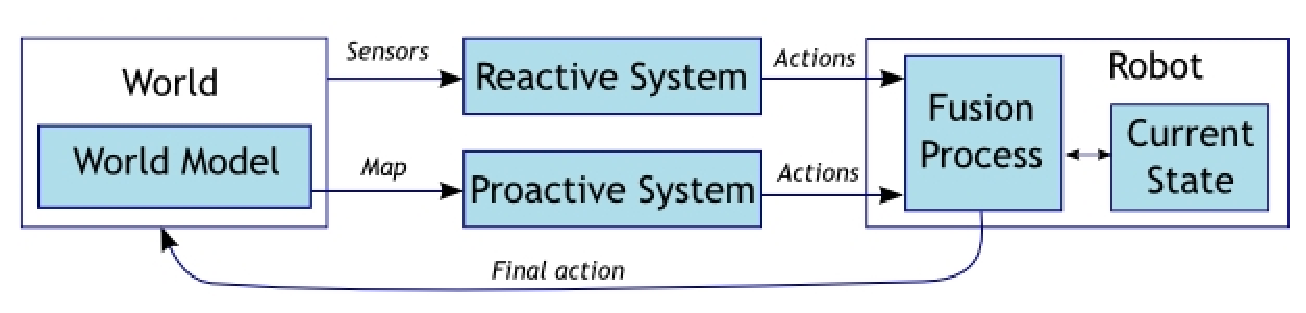
\includegraphics[width=0.8\textwidth]{imgs/img-scheme.eps}
	\caption{\label{fig:hybrid} Hybrid scheme for a robotic system.}
\end{figure}

In this picture the world is the real environment. The world model is a map containing the static elements of the environment. The reactive system is made of several generators, for the sensors and for the user's orders. The proactive system is the AI of the robot. The robot is the only actor in the system. The current state is the set of robot attributes. The multisensorial integration process is the evolution function of the robot. The final action is the result of the process of sensor integration and the final action carried out by the robot.


Only one primitive is needed, the robot, and it is modified by two possible transformations: move and rotate (table \ref{tab:PrimTransf}). When the system is executed in a real environment, the transformations correspond to the actual operations performed by the robot. If it is executed in a simulator, the primitive and the transformations will represent the operations carried out in the graphics system (GS).

\vspace{-0.3cm}
\begin{table}[h]
\begin{center}
\begin{tabular} {|l|l|l|}
\hline
	 & Real environment & Simulator \\
\hline
	$PRobot$ & No action & Draw the robot in the GS \\
\hline
	$TMove_{<dist>}$ & Move a distance $dist$ & Move a distance $dist$ in the GS \\
\hline
	$TRotate_{<angle>}$ & Rotate an angle $angle$ & Rotate an angle $angle$ in the GS \\
\hline
\end{tabular}
\end{center}
\caption{Primitives and transformations of the robotic system.}
\label {tab:PrimTransf}
\end{table}


Events are used to define the activity in the system. Each event is defined by its identifier and some attributes. They produce changes on the actors through their evolution functions. 
These events are produced by generators. There is a generator for each event type. In the robotic system, five generators are needed:

\begin{itemize}
	\item \textit{gLaser}: It generates an \textit{eLaser} event when the laser detects an obstacle, 
			by obtaining the laser data and processing them to find the possible obstacles.
			It is defined as: 
			$gLaser$ = $eLaser_{<dist,angle>}$  if obstacle, where
			$dist$ is the distance to the obstacle and $angle$ is the angle to the obstacle.
			
	\item \textit{gCamera}: It generates an \textit{eCamera} event when a marker is detected in the camera image. 
			Markers are used to identify the rooms in the environment.
			It is defined as:			
			$gCamera$ = $eCamera_{<marker>}$ if a marker is detected. 
			
	\item \textit{gDecide}: It generates an \textit{eDecide} event each frame to 
			indicate to the robot to make a decision. 
			Is is defined as: 	
			\textit{gDecide = eDecide} each frame.
			
	\item \textit{gExecute}: It generates an \textit{eExecute} event to indicate the system 
			to execute the robot actions in the current representation space. 
			If the representation space is the real environment, 
			the real operations will take place (move the robot, rotate the robot...). 
			If the current space is the simulator, the operations will take place in the graphics system. 
			It is defined as:			
			\textit{gExecute = eExecute} each frame.
			
	\item \textit{gObjective}: It generates an \textit{eObjective} event to set a new objective marker. 
			This generator is connected to the user orders. Users can specify a new target room 
			simply by selecting its associated marker.
			It is defined as: 
			$gObjective$ = $eObjective_{<marker>}$ if user order.

			
\end{itemize}

An order relation must be defined to establish an execution priority among generators. In the robotic system, the order relation is: \textit{gLaser, gCamera, gObjective, gDecide, gExecute}. Therefore, events related with the acquisition of data have the highest priority, compared with the events of decision and execution.




% \subsubsection{Actors}
The only actor in our robotic system is the robot which is defined as:

$ARobot^{eLaser, eCamera, eDecide, eExecute, eObjective}_{<grid, row, column, angle, objective, action>}$, 
where the superscript are the events which it is prepared to respond to, and the subscript are the attributes, whose meanings are: 
the \textit{grid} represents the environment where the robot moves in. 
	Each cell stores the registered data obtained from the sensors (the detected obstacles and markers).
\textit{Row and column} are position occupied by the robot in the grid.
\textit{Angle} is the robot orientation.
\textit{Objective} is the objective room, represented by its marker.
And \textit{action} is the string of primitives and transformations which 
	indicates the next command to be executed.
To simplify, in the following equations this actor will be referred as $ARobot^{E}_{<g, r, c, an, o, ac>}$.

The evolution function defines the way the robot behaves in the environment. Let $e$ be an event that is received by the actor, the evolution function is defined as:

\vspace{-0.4cm}
\begin{equation}
	\begin{small}
	\lambda (ARobot^{E}_{<g, r, c, an, o, act>}, e)= 
    \left\{
    \begin{array}{ll}
		ARobot^{E}_{<g', r, c, an, o, ac>} & \mathit{if}  \ \ e = eLaser_{<dist,angle>} \\ 
        ARobot^{E}_{<g', r, c, an, o, ac>} & \mathit{if}  \ \ e = eCamera_{<marker>} \\ 
        ARobot^{E}_{<g, r', c', an', o, ac'>} & \mathit{if}  \ \ e = eDecide \\ 
        \alpha(ARobot^{E}_{<g, r, c, an, o, ac>}) & \mathit{if}  \ \ e = eExecute \\ 
        ARobot^{E}_{<g, r, c, an, o', ac>} & \mathit{if}  \ \ e = eObjective_{<marker>} \\ 
        ARobot^{E}_{<g, r, c, an, o, ac>} & otherwise
    \end{array}\right.    
	\end{small}
\end{equation}

where the symbol apostrophe (') indicates that it has changed as follows:


\begin{itemize}
	\item If $e=eLaser_{<dist,angle>}$, the grid ($g$) must be updated 
			to indicate that an obstacle has been detected. The cell to
			mark is the one in position $(r+dist\ \cos(ang+angle), c+dist \ \sin(ang+angle))$.
			
	\item If $e = eCamera_{<marker>}$, the grid must be updated to indicate 
			that a marker has been detected. The cell to mark is 
			$(r+dist \ \cos(ang), c+dist \ \sin(ang))$.
			
	\item If $e = eDecide$, the current position and orientation of the robot ($r, c, ang$), 
			must be updated, as well as the actions to be executed. 
			
	\item If $e = eExecute$, the actions of the robot must be executed in the representation space, 
			through the use of the $\alpha$ function.
			
	\item If $e = eObjective_{<marker>}$, a new objective has been set by the user, 
			so the objective ($o$) must be changed to the new one ($marker$).
			
	\item In any other case, the actor must remain unchanged.
			
\end{itemize}


%--------------------------------------------------------------------------
%\subsubsection{Initial string}

The initial string in our system is defined as: 
$ARobot^{eLaser, eCam., eDecide, eExec., eObjct.}_{<grid, row, column, angle, \epsilon, \epsilon>}$, 
where the attribute grid is initialized to a set of empty cells, 
the attributes row, column and angle are the initial position, 
and the objective and the actions are empty.



%--------------------------------------------------------------------------
\subsection{Analysis}

A set of tests has been designed to prove the features of our model:
The aim of the first test is to prove the suitability of the evolution function to introduce new AI algorithms. 
This test is not to obtain the best AI algorithm to achieve the goal. 
Two simple decision algorithms have been used to decide how the robot should move. The first algorithm makes decisions randomly to find the target position. The second algorithm is A* \cite{Luo2010}.
These two AI algorithms were introduced without making any changes in other parts of the system, 
just by changing the evolution function. 


%--------------------------------------------------------------------------
%\subsubsection{Test of device independence}
The aim of the second test is to prove that the input devices can be replaced without changing the system. We can change the laser to a Kinect to detect obstacles. To change this device, we have just designed a new event generator (\textit{gKinect}) that creates events of the same type that the ones generated by the laser generator.


%--------------------------------------------------------------------------
%\subsubsection{Test of the system extensibility}
In the third test we want to test the extensibility of the system. New instances of the actor symbols (representing robots) have been added to the definition string to extend the system and create a multi-robot system in an almost immediate way. The updating of the definition string supposes the extension of the model and the addition of new features. Moreover, most elements can be reused in new definition strings to obtain new behaviours with little effort.

%--------------------------------------------------------------------------
%\subsubsection{Test of changes in the environment}
In the last experiment we tested the flexibility to work under different conditions. To prove this feature, the system has been tested with different maps, in the case of the simulated robot, and in different real environments, in the case of the real robot.

%\vspace{-0.4cm}
%\begin{figure}
%	\centering
%	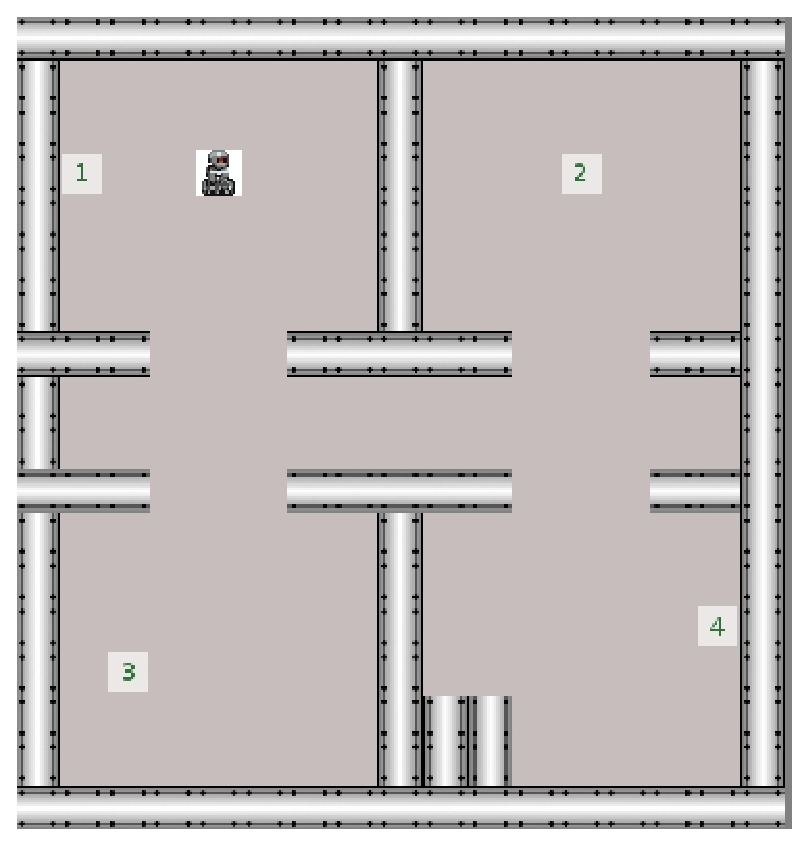
\includegraphics[width=2cm]{imgs/mapa.eps} \ \ \ \ \ \ \ \ \ \
%	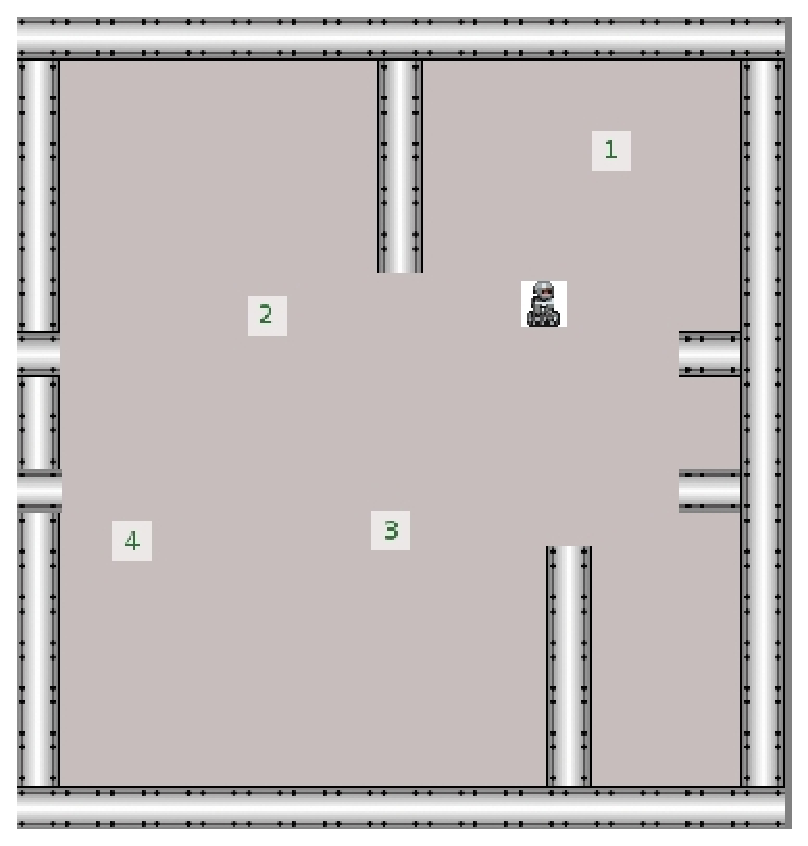
\includegraphics[width=2cm]{imgs/mapa2.eps}
%	\caption{\label{fig:maps} Two example maps.}
%\end{figure}



%--------------------------------------------------------------------------
\section{Conclusions}
%--------------------------------------------------------------------------

A new model to formally define virtual worlds, independently from the underlying physical layer, has been presented. Is has been used to model the control of a mobile robot, navigating in a given environment, and using a set of multimodal inputs from different types of sensors.

Taking into account the diversity of virtual worlds available nowadays and the wide variety of devices, this model seems to be able to provide interesting features. Firstly, it is a formal model that allows to abstract and represent the states of the system in a general way by avoiding specific features. It is a device-independent model, therefore, is not linked to the implementation. It allows the replacement of physical devices by simulated ones, and the easy addition of new ones.

In conclusion, it has been achieved the main objective of defining a new formal and generic model that is able to model general virtual worlds systems by avoiding the specific peculiarities of other models existing today.

% -----------------------------------------------------------------
% Bibliografa //Para bibtex
% -----------------------------------------------------------------
%\bibliographystyle{named}
%\bibliography{ref}

\begin{thebibliography}{0}

%\bibitem{Botts2006}     %%%%%%NUEVO%%%%%%
%Botts, M.; Percivall, G.; Reed, C. and Davidson, J.:
%OGC Sensor Web Enablement: Overview And High Level Architecture. 
%OGC White Paper. Open Geospatial Consortium Inc., (2006)


\bibitem{Davis1994}
Davis, Martin; Sigal, Ron and Weyuker, Elaine J.:
Computability, Complexity, and Languages, Fundamentals of Theoretical Computer Science, 2nd~ed.
San Diego: Elsevier Science (1994)


\bibitem{Ernst2004}         %%%%%%%%%NUEVOOO%%
Ernst, Marc O. and B\"{u}lthoff, Heinrich H.:
Merging the senses into a robust percept.
TRENDS in Cognitive Sciences, vol.8, no.4, ( 2004)


\bibitem{Ingrand2001}  %%%%%NUEVO%%%%
Ingrand, F.; Chatila, R.  and Alami, R.:
An Architecture for Dependable Autonomous Robots. 
IARP-IEEE RAS Workshop on Dependable Robotics (2001)

\bibitem{Luo2010}  %%%%%%%A*
Luo, Ren; Lin, Yu-Chih; Kao, Ching-Chung:
Automous mobile robot navigation and localization based on floor paln map information and sensory fusion approach. 
IEEE MFI (2010)

\bibitem{Posadas2008} %%%%%%NUEVO%%%
Posadas, J.L.; Poza, J.L., Sim\'{o}, J.E.; Benet, G.; Blanes, F.:
Agent-based distributed architecture for mobile robot control. 
Engineering Applications of Artificial Intelligence, 805-823 (2008) 

%\bibitem{Poza2008}  %%%%%NUEVO%%%%
%Poza, L.; Posadas, J.; Sim\'{o}, J.; Benet, G.:
%Arquitecturas de control jer\'{a}rquico inteligente con soporte a la calidad de servicio. 
%XXIX Jornadas de Autom\'{a}tica (2008)


%%%%%NUEVOOOOOOO
\bibitem{Russell2010}       %%%%%%%%%
Russell, Stuart Jonathan and Norvig, Peter:
Artificial intelligence: a modern approach.
Prentice Hall. ISBN: 0136042597. (2010)


\bibitem{Sharma1998}  %%%%% NUEVO %%%%
Sharma, R.; Pavlovic, V. I.; Huang, T. S.:
Toward Multimodal Humar-Computer Interface.
Proceedings of the IEEE, vol. 86(5), pp. 853-869 (1998)

\bibitem{Singhal1997}  %%%%% NUEVO %%%%
Singhal, A.; Brown, C.:
Dynamic bayes net approach to multimodal sensor fusion. 
SPIE 1997


%\bibitem{Weser2008}        %%%%%%%NUEVO%%%%
%Weser, Martin ; Jockel, Sascha  and Zhang, Jianwei:
%Fuzzy Multisensor Fusion for Autonomous Proactive Robot Perception
%IEEE International Conference on Fuzzy Systems (FUZZ),  2263-2267 (2008)



\end{thebibliography}

\end{document}

%%
